\documentclass[openany]{book}
\usepackage{titlesec,titletoc,indentfirst,amsmath,amssymb,amsthm,amsfonts,mathtools,enumitem,graphicx,fancyhdr,environ,setspace,tikz}
\usepackage[dvipsnames]{xcolor}
\usepackage[most]{tcolorbox}
\usepackage[a4paper,top=3cm,bottom=2cm,right=2cm,left=2cm]{geometry}
\NewEnviron{remark}[1][]{\begin{tcolorbox}[colback=Cerulean!5!white,colframe=Cerulean!60!white,fonttitle=\bfseries,title=Remark {#1}]\singlespacing\vspace{-0.5cm}\BODY\end{tcolorbox}}
\NewEnviron{definition}[1][]{\begin{tcolorbox}[colback=LimeGreen!5!white,colframe=LimeGreen!60!white,fonttitle=\bfseries,title=Definition {#1}]\singlespacing\vspace{-0.5cm}\BODY\end{tcolorbox}}
\NewEnviron{formula}[1][]{\begin{tcolorbox}[colback=Emerald!5!white,colframe=Emerald!60!white,fonttitle=\bfseries,title=Formula {#1}]\singlespacing\vspace{-0.5cm}\BODY\end{tcolorbox}}
\NewEnviron{example}[1][]{\begin{tcolorbox}[colback=DarkOrchid!5!white,colframe=DarkOrchid!60!white,fonttitle=\bfseries,title=Example {#1}]\singlespacing\vspace{-0.5cm}\BODY\end{tcolorbox}}
\NewEnviron{theorem}[1][]{\begin{tcolorbox}[colback=MidnightBlue!5!white,colframe=MidnightBlue!60!white,fonttitle=\bfseries,title=Theorem {#1}]\singlespacing\vspace{-0.5cm}\BODY\end{tcolorbox}}
\NewEnviron{property}[1][]{\begin{tcolorbox}[colback=Rhodamine!5!white,colframe=Rhodamine!60!white,fonttitle=\bfseries,title=Property {#1}]\singlespacing\vspace{-0.5cm}\BODY\end{tcolorbox}}
\newcommand{\secmark}{}
\newcommand{\marktotoc}[1]{\renewcommand{\secmark}{#1}}
\newenvironment{advanced}
{\renewcommand{\secmark}{\dag}
\addtocontents{toc}{\protect\marktotoc{\dag}}}
{\addtocontents{toc}{\protect\marktotoc{}}}
\usetikzlibrary{patterns,patterns.meta}
\setlength{\headsep}{0.5cm}
\setlength{\parindent}{20pt}
\onehalfspacing
\title{Spring 2026 Tutoring Notes}
\author{Austin Kim}

\titleformat{\chapter}
	{\LARGE}{\textbf{\llap{\secmark\hspace{0.2cm}}Chapter \thechapter}\\}{1em}{}
\titlespacing{\chapter}
	{0pc}{3.5ex plus 0.1ex minus 0.2ex}{1.5ex minus .1ex}
\titlecontents{chapter}[20pt]{}
	{\Large\contentslabel[\textit{\textbf{\llap{\secmark\thecontentslabel}}}]{10pt}}{}{}

\titleformat{\section}
	{\Large}{\textbf{\llap{\secmark\hspace{0.2cm}}\thesection}}{1em}{}
\titlespacing{\section}
	{0pc}{3.5ex plus 0.1ex minus 0.2ex}{1.5ex minus .1ex}
\titlecontents{section}[42pt]{}
	{\contentslabel[\textit{\llap{\secmark\thecontentslabel}}]{10pt}}{}{}

\titleformat{\subsection}
	{\large}{\textbf{\llap{\secmark\hspace{0.2cm}}\thesubsection}}{1em}{}
\titlespacing{\subsection}
	{0pc}{3.5ex plus 0.1ex minus 0.2ex}{1.5ex minus .1ex}
\titlecontents{subsection}[64pt]{}
	{\contentslabel[\textit{\llap{\secmark\thecontentslabel}}]{10pt}}{}{}
\begin{document}
\maketitle

\setlength{\headsep}{0.5cm}
\section*{Foreword}
\normalsize \indent hello!! :3 \vspace{0.6cm}\\
austin kim

\tableofcontents
\chapter{Numbers}
\section{Preliminaries}
Before we begin our work on defining numbers, it is important to ask why we should care at all about the particular labor that we are about to undertake. This is a fairly good habit; a student should always ask why they should care about anything that follows. It highlights the importance of what we are learning, and a good answer to such a question will also define a relation between things that we already know and the things we are about to learn.\par
Numbers are a majority of where we start our study of mathematics. They are the motivation for all of mathematics --- we use them to count dumplings, tell people how much money we made, and tell our parents we have only been goofing off for 30 minutes, not 50, and that we will get back to doing homework soon enough (does every mother say that it's `almost 11' when it's actually just 10:15? How is that at all close to 11???). However, it is not always obvious how these numbers work: our counting numbers are very natural ideas; we are born and immediately have the concept of having ten toes or six siblings. The following ideas, such as fractions and decimals, are a lot less simple, and they warrant some extra study and formal introduction. In fact, even the natural numbers and integers have certain virtues and weaknesses that are not always immediately obvious.\par
All of this is to say that it is actually worth speaking about numbers at a more sophisticated level than waving our hands and saying, ``well, they are what they are, and everyone knows how they act." I hope that by the end of this section, the reader develops at least some appreciation for the complexity and often strange nature of numbers. Let's begin!
\section{Natural and Whole Numbers}
\begin{definition}[(Natural Number, $\mathbb{N}$)]
	A natural number $n$ is essentially a counting number --- think of our familiar numerals 1, 2, 3, 4, etc. These proceed infinitely; as far as you can count, that number will still be a natural number. In particular, the group of natural numbers $\mathbb{N}$ (this is the symbol for the entire group of natural numbers) is infinite.
\end{definition}
\begin{remark}
	It may help to observe that we start at 1, add 1, and continue doing so. This produces every single natural number: we say that if $n$ is a natural number, the next natural number is of the form $n+1$. An example of this is that 5 is obviously a natural number, and by adding 1 to it and having $5+1=6$, we produce another natural number!
\end{remark}
\begin{definition}[(Whole Number)]
	There is very little exciting new material here, unfortunately. A whole number $m$ is simply either a natural number or 0.
\end{definition}
We can observe that natural and whole numbers are able to do all of the nice operations of addition, subtraction and multiplication. We may also define a new set of numbers, though, using the idea of subtraction. In particular, we want to have a way to express that some numbers can be \textit{negative} --- in some sense, the opposite of addition! First, we will discuss some vocabulary that will be useful as we move forward.

\section{Integers and a Few Useful Words}
\begin{definition}[(Inverse)]
	This is more of an English vocabulary definition than a mathematical definition. An inverse is something like the opposite of something else, or something that undoes something else.
\end{definition}
\begin{example}[(Inverse)]
	One might say that the inverse of red is blue, or that the inverse of light is dark. Within the context of math, we may say that the inverse of addition is subtraction, and that the inverse of multiplication is division. Since the negative version of a number $n$, $-n$, has the property that $n+(-n) = n-n = 0$, we call $-n$ the ``additive inverse" of $n$. Similarly, for multiplication, since any number $n$ has that $n\cdot\dfrac{1}{n}=1$, we say that $\dfrac{1}{n}$ is the ``multiplicative inverse" (long words, unfortunately) of $n$.
\end{example}
\begin{definition}[(Integer, $\mathbb{Z}$)]
	An integer $n$ is a number that is either a whole number or its negative version (the additive inverse!). The set of integers is written $\mathbb{Z}$.
\end{definition}
It is useful to note that we are now able to fully perform addition and subtraction with no worries about `going outside' of our number system! For example, previously, if we asked about the result of a computation such as $2-3$, we would be left wondering what exactly could possibly be the result. However, now, we can safely claim that it is $-1$, and the integers are what allow this.\par
However, we run into some problems when we move to division: we cannot produce answers to seemingly possible operations such as $2\div3$. This gives us motivation to define an even larger set of numbers with a new entry, the fraction. Here we will call this system the `rational numbers,' written as $\mathbb{Q}$.

\section{The Rational Numbers}
\begin{definition}[(Rational Number, $\mathbb{Q}$)]
	A rational number $r$ is a number of the form $\dfrac{p}{q}$, where $p$ and $q$ are integers.
\end{definition}
We usually want to reduce this fully. For example, we can say $\dfrac{2}{6}$ is a rational number, and that is entirely true, but we would really like to call it $\dfrac{1}{3}$ $\left(\text{to see how this happens, multiply }\dfrac{2}{6}\text{ by }\dfrac{\frac{1}{2}}{\frac{1}{2}}\right)$.\par
Well, rationals are \textit{very} nice: within the rational numbers $\mathbb{Q}$, we can add and subtract freely without going outside of our number system, since every rational number has its additive inverse: if we have a rational number $\dfrac{p}{q}$, we also have the rational number $\dfrac{-p}{q}$, since $-p$ is still an integer, so we are still talking about a rational number. In fact, a similar thing is true for multiplication now: if I have a rational number $\dfrac{p}{q}$ and we multiply it by $\dfrac{q}{p}$, which is obviously another rational number since both $q$ and $p$ are integers, we get 1!
\section{Let's Talk About Fractions and Decimals!}
So... what is a decimal, then? We talked about rational numbers, and it seems like there are a \textit{LOT} of them, but we still have not discussed decimals.\par
\begin{definition}[(Numerator, Denominator)]
	In a rational number $r = \dfrac{p}{q}$, the numerator is $p$ and the denominator is $q$.
\end{definition}
For the most part, fractions will suffice. Daily life, ranging from cooking pasta to splitting pies will all call for fractions. However, decimals are not without their uses. In fact, we can represent any fraction as a decimal, even if it has to go on forever! This can be observed easily on a calculator simply by dividing the numerator by the denominator. The result should be a decimal.\par
This means something very important: every fraction can be converted to a decimal if we need to do so. The fact that these decimals are truly equal to their fraction counterparts can be observed by adding and multiplying with them to show that they behave exactly as the fraction should. For example, $0.5$ will be seen to act exactly as $\dfrac{1}{2}$ does, where adding it to itself results in $1$, and multiplying it by $2$ gives $1$ as well.\par
However, decimals are actually a \textit{larger} system of numbers than fractions (or, in our fancy words, rational numbers) are. This delves a bit into forbidden territory, but we shall address it anyway after a short excursion to pictures.

\section{A Few Diagrams for the Visual Learner}
Well, how can we visualize any of this? There is some good news: numbers, as strange as they are, can be placed on the familiar number line, and the way that we can see this is shown below. \vspace{0.4cm}
\begin{center}
	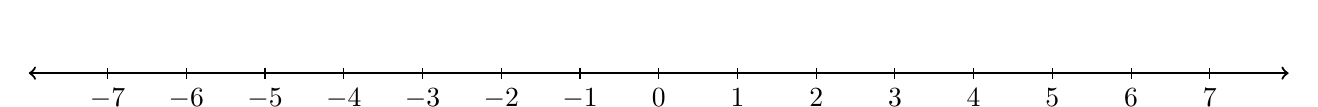
\begin{tikzpicture}
		\draw[step=1cm,black,thick,<->](-8,0) -- (8,0);
		\foreach \x in {-7,...,7}
			\draw (\x cm, 2pt) -- (\x cm,-2pt) node[anchor=north] {$\x$};
	\end{tikzpicture}
\end{center}\par
Here we see the integers from -7 to 7. There is nothing very shocking about this; we have investigated this before. The integers, of course, extend infinitely into the negatives and positives. However, the next things to discuss are the rational numbers, and these are actually impossible to draw. Why? Well, consider just the fractions between 0 and 1. What we find out is that any fraction $\dfrac{1}{n}$ where $n$ is some natural number is positive, so it is greater than 0, but since we know that the larger the denominator, the smaller the fraction is, we realize that any fraction $\dfrac{1}{n}$ where $n \geq 2$ is immediately smaller than 1.\par
Why does this matter? Well, the upshot is that we can stuff \textit{infinite} fractions between just 0 and 1: write any number $\dfrac{1}{n}$ and be assured that it is between 0 and 1, and since there are infinite natural numbers, there are infinite fractions of that form! However, we can still think of the rationals as adding some `filling' between every integer. And since we see that there are infinite fractions between 0 and 1, and similarly there are infinite fractions between any two integers, the rationals actually add a \textit{massive} amount of `filling!'
\begin{center}
	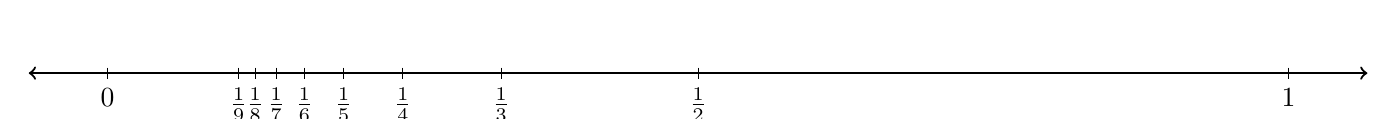
\begin{tikzpicture}
		\draw[step=1,black,thick,<->](-1,0) -- (16,0);
		\draw (0,2pt) -- (0,-2pt) node[anchor=north] {$0$};
		\foreach \x in {0,2,4,6,8,10,12,14}
			\pgfmathtruncatemacro{\varA}{18-\x}
			\pgfmathtruncatemacro{\varB}{\varA/2}
			\draw (30/\varA, 2pt) -- (30/\varA,-2pt) node[anchor=north] {$\frac{1}{\varB}$};
		\draw (15,2pt) -- (15,-2pt) node[anchor=north] {$1$};
	\end{tikzpicture}
\end{center}\par
We can see above the idea of stuffing a bunch of rational numbers in between whole integers. In fact, if we are creative, we can make even \textit{more} filling by taking any two rational numbers $\dfrac{p_{1}}{q_{1}},\dfrac{p_{2}}{q_{2}}$, adding them, and dividing them by two to find the rational number in the middle of them. This usually returns a very ugly number $\left(\text{in particular, it is written }\dfrac{p_{1}q_{2}+p_{2}q_{1}}{2p_{2}q_{2}}\right)$, but we can actually simply think about why this should still be a rational number: we remember that the `good' part of rational numbers is that any two rational numbers added or multiplied together is still a rational number, so surely adding two rational numbers then dividing them by two, which is also multiplying by $\dfrac{1}{2}$, should give us another rational number.

\section{Some Forbidden Numbers: The Irrational Number System}
So... what is an `irrational number,' then? Is it a number that makes no sense?\par
Sort of.
\begin{definition}[(Irrational Number)]
	An irrational number is a decimal number that has infinite decimals but has no pattern. For example, 0.1111111... is not irrational because there is a clear pattern: every decimal digit is 1! Even something like 0.142142142142142... is not irrational because the 142 keeps repeating.\par
	However, a number like $\pi=3.14159265358979323846...$ is irrational because there is absolutely no clear way to understand what will show up next.\par
	In particular, \textit{an irrational number CANNOT be written as a rational number}, that is, we cannot write an irrational number as a fraction $\frac{p}{q}$ where $p,q$ are integers.
\end{definition}
\begin{remark}
	The first definition given above for irrational numbers is technically not the actual mathematical definition of an irrational number. That title would have to go to the last sentence of the definition; it is simply a real number that cannot be written as a fraction of two integers. However, for daily purposes, the first definition completely suffices.
\end{remark}
The important part here is to note that the existence of irrational numbers shows that even though every fraction can be written as a decimal, not every decimal can be written as a fraction. Still, though, since we understand decimal numbers as ``numbers between integers," we can also see that irrational numbers are part of our `fillings' between integers. For example, the number $\pi$ is greater than 3 but less than 4, so it lies somewhere between the two.\par
This concludes, for now, our study of different types of numbers. There is a very abstract idea about why this is the temporary stopping point for our definitions of numbers, but that is significantly too advanced for even notes such as this. It essentially boils down, however, to the idea given above: that we have finished filling in the blank spaces between our integers.

\section{Exercises}
Every student must complete exercises, and many of them, in order to fully understand the mathematics that they are learning. I, myself, have tried to dodge these exercises as they are often difficult and sometimes dry. However, it is unfortunately a fact that practice must be done in order to improve at anything. I hope that the reader will understand this necessity and complete at least half of these exercises. Bold-faced problems are exceptionally difficult and pose genuine problem-solving exercises; these will not be found in every exercise section, and they often hinge on the reader having read and understood the optional difficult sections. The rest of the exercises are largely small recitations of definitions or checks to show that the reader has thoroughly read and understood all of the definitions and examples.
\begin{enumerate}
	\item Give six examples of natural numbers.
	\item Give an example of a whole number that is \textit{not} a natural number.
	\item How many natural numbers are whole numbers? \textit{Hint: there is an infinite number of natural numbers.}
	\item State the definition of a rational number.
	\item \textbf{Explain the relationship between fractions and rational numbers. Which fractions are rational numbers, and which rational numbers are fractions? Are there fractions that are \textit{not} rational numbers, or rational numbers that are \textit{not} fractions?}
	\item \textbf{Is every rational number able to be written as a decimal? Is every decimal able to be written as a rational number? If not, either give an example that defends your answer, or intuitively explain why the statement is false.}
\end{enumerate}

\chapter{Operations}
\section{Preliminaries}
Numbers are fine and well, but we would really also like to know what to do with them. In a vacuum, these numbers do nothing, and the natural thing to do is to look for actual usages of them. Here operations come into play, and these are quite familiar. Addition, subtraction, multiplication, and division are our familiar friends, and in later studies, the reader will see many other, more complex operations (exponentiation, logarithms, and more).\par
An important idea to note is that while we can do many of these operations at once, at their core, these operations are `binary': they take in two entries and spit one result out. For example, when we add, we need to add two numbers, and only one number comes out. In a sense, binary operations are a little machine that accepts two coins and produces one coin. Perhaps we enter the numbers 6 and 3 and our machine produces 9. Or we can enter 6 and 3 and our machine produces 2 (if the machine in question is division)!\par
These operations become more and more complex as we do many of them in a row and also ask what happens if we do certain operations together. In general, we should like to group these operations into pairs anyway: for example, we can write $2+3+4+5+6+7$, but in reality, what we are actually doing is performing the operation $2+3$, then taking the result of 5 and performing $5+4$, then taking \textit{that} result and computing $9+5$, and this process continues until we are done. All of this is to say that our operations are truly just two numbers somehow becoming one in different ways.\par
As for the motivation for studying operations, it is rather obvious that operations give life and depth to the numbers: one may simply count how many candies are in their bag, or they can add the number of candies that they and their friends have in order to find the total number of candies. Such operations truly make numbers useful and thus warrant concentrated and special study.
\section{Addition}
\subsection{Properties of Addition}
Addition has a few very nice properties. They are as follows:
\begin{property}[(Associative Property of Addition)]
	For any three real numbers $a,b,c$, we have
	\begin{center}
		$(a+b)+c = a+(b+c)$.
	\end{center}
\end{property}
\begin{property}[(Commutative Property of Addition)]
	For any two real numbers $a$ and $b$, we have
	\begin{center}
		$a+b = b+a$.
	\end{center}
\end{property}
\begin{property}[(Identity Property of Addition)]
	For any real number $a$, we have
	\begin{center}
		$a+0=a$.
	\end{center}
\end{property}
\begin{property}[(Inverse Property of Addition)]
	For any real number $a$, we call the negative number $-1\cdot a = -a$ the `additive inverse' of $a$ and write
	\begin{center}
		$a+(-a)=0$.
	\end{center}
\end{property}
These should simply be accepted as fact, but if there is any confusion about them, the reader may simply appeal to intuition and usage of integer examples.
\subsection{Addition on Fractions}
Fractions, particularly the rational numbers $\mathbb{Q}$ as previously discussed, give us a way to describe some of the numbers that lie between integers. They, along with the irrational numbers, fill our real number line completely. Then it follows that we should be curious about how to add and multiply these numbers. This is the object of our current investigation.\par
It is useful to think of fractions as a `slice' of a whole --- a pie, a paper, or whatever else may suit the reader. Indeed, adding fraction sof like denominators is trivial: we simply say that the numerator increases by normal addition. This intuitively makes sense: if we have $\dfrac{1}{n}$, this is something akin to saying that we have split 1 whole into $n$ equal, or `congruent,' parts. Then if we have multiple of these together, say perhaps $\dfrac{1}{n}+\dfrac{2}{n}$, we should surely have three of those even slices. In general, we will codify this as follows.
\begin{theorem}
	For any two fractions with identical denominators $\dfrac{p_{1}}{q}$ and $\dfrac{p_{2}}{q}$, their sum is computed as
	\begin{center}
		$\dfrac{p_{1}}{q}+\dfrac{p_{2}}{q} = \dfrac{p_{1}+p_{2}}{q}$,
	\end{center}
	that is, when two fractions have the same denominator, the addition follows by simply adding their numerators. In fact, none of $p_{1},p_{2},q$ need to be rational for this to be true.
\end{theorem}
\begin{example}
	Suppose we want to add $\dfrac{34}{3}$ and $\dfrac{24}{3}$. Our formula essentially implies that we need only think about adding the slices, and our intuition says that this should obviously result in 58 even slices, each a third of 1 whole. Indeed, we compute $\dfrac{34}{3}+\dfrac{24}{3}=\dfrac{34+24}{3}=\dfrac{58}{3}$, and we are done.
\end{example}
This is likely very familiar to the reader, but a difficulty arises when we must add two fractions of unlike denominators, e.g. $\dfrac{1}{3}$ and $\dfrac{2}{5}$. To solve this, suppose we attempt to apply our theorem and write $\dfrac{1}{3}+\dfrac{2}{5}=\dfrac{1+2}{5}$. This is clearly suspicious because we have randomly chosen 5 to be our denominator --- what stops us from randomly picking 3? And does this make any sense, to begin with? $\dfrac{1}{3}$ is clearly larger than $\dfrac{1}{5}$, being only 3 times smaller than 1 whole while the fifth is 5 times smaller. So how could adding $\dfrac{1}{3}$ to $\dfrac{2}{5}$ result in adding $\dfrac{1}{5}$? It is clear that our previous theorem that makes fraction addition so easy unfortunately no longer applies here.\par
To solve this problem, we can think of each fraction being spoken in some language defined by its denominator. Attempting to add fractions of different denominators fails in the same way that a Korean-speaker would fail to hold conversation with a Russian-speaker. Then, as with language, we should translate these denominators to the same `language,' a \textit{common denominator}.\par
Well, let us attempt to do so on our previous problem. I will pick 5 to be our common denominator... but there is no clear way to convert thirds into fifths! So clearly we need to try harder; our method will be as follows: we will find a number which both 3 and 5 can divide, namely $3\times5=15$. Why? Well, this allows for clean translation of both the thirds and fifths because all we need to do is scale the numerator of the fraction by the proper factor. For example, when 5 turns to 15, we have made the denominator 3 times larger, so we should also make the numerator 3 times larger. Then $\dfrac{2}{5}$ becomes $\dfrac{6}{15}$, and similarly, since 3 becomes 5 times larger to become 15, $\dfrac{1}{3}$ becomes $\dfrac{5}{15}$. Then our fraction addition becomes much simpler; our previous theorem applies to it and we obtain $\dfrac{2}{5}+\dfrac{1}{3}=\dfrac{6}{15}+\dfrac{5}{15}=\dfrac{11}{15}$, and we are done.\par
In general, we can say that we add fractions by ensuring that they have the same denominator, either because they do to begin with or because we simply multiply one fraction in both the numerator and denominator by the other fraction's denominator.
\begin{example}
	Suppose we would like to add $\dfrac{13}{15}$ and $\dfrac{21}{19}$. We see that the denominators are different, so we would like to find a number that both 15 and 19 may cleanly divide so that our numerators are clean as well. It is guaranteed that both 15 and 19 can divide $15\times19$, so we will make our common denominator 285. Then, to change each fraction to having the proper denominator, we multiply $\dfrac{13}{15}$ in the numerator and denominator by 19, and we multiply $\dfrac{21}{19}$ in the numerator and denominator by 15. This produces $\dfrac{13}{15}+\dfrac{21}{19}=\dfrac{247}{285}+\dfrac{315}{285}=\dfrac{247+315}{285}=\dfrac{562}{285}$.
\end{example}
\begin{remark}
	At this point, it may be understandable why we want to find a common denominator, but the reader may still be confused on why we do what we do in order to find a common denominator, and why such a technique is actually mathematically allowed. This can be explained by the fact that any number divided by itself is 1.\par
	We see above that by multiplying $\dfrac{13}{15}$ in the numerator and denominator by 19, what we are really doing is computing $\dfrac{13}{15}\cdot\dfrac{19}{19}$. This must preserve equality because we are multiplying by 19 divided by itself, which must be 1, and any number multiplied by 1 is itself. Then by doing the analogous technique on $\dfrac{21}{19}$, we have converted the two fractions into fractions of like denominators while preserving their values.\par
	In some sense, what we have computed is actually just $\dfrac{13}{15}\cdot1+\dfrac{21}{19}\cdot1$, and of course this is equal to the original expression.
\end{remark}
This finishes our addition on fractions; we have now learned how to add fractions of like and unlike denominators. Of course, for addition of fractions with negative numerators, all we need to do is observe that after our denominators agree, the numerators become $p_{1}+p_{2}$, and this is simply integer addition, as demonstrated in Section 2.1.1.
\subsection{Addition on Decimals}
Addition of decimals is executed in a rather simple way: one only needs to observe that the decimal points are placed correctly. This is done as follows: suppose we want to compute $0.34+12.1429$. If we simply add 4 to the 9 and add 3 to the second 2, we will end up with a completely incorrect answer because we are adding numbers in the incorrect tenths places. Instead, if we `line up' the decimals and compute
\[
\begin{array}{@{}cl}
	&12.1429 \\
	+&00.34\\
	\cline{2-2}
	&12.4829
	\end{array}.
\]
then the correct answer follows.\par
Some confusion is warranted on why this problem-solving technique in particular is correct. This is best explained with integers: suppose we are asked to add 63 and 1, and instead of adding the 3 by 1, we instead shift the 1 to the left, like so:
\[
\begin{array}{@{}cl}
	&63\\
	+&1\\
	\cline{2-2}
	&73
\end{array}.
\]\par
This clearly produces a `bad' answer; the problem is, of course, that 1 is not 10, and so it is being added to the wrong tens place when computed as shown. Indeed, we should have
\[
\begin{array}{@{}cr}
	&63 \\
	+&1\\
	\cline{2-2}
	&64
\end{array}.
\]\par
Similarly, when we add 0.34 and 12.1429, instead of writing
\[
\begin{array}{@{}cr}
	&12.1429 \\
	+&0.34\\
	\cline{2-2}
	&12.1463
	\end{array},
\]
we should instead line the decimals up to create
\[
\begin{array}{@{}cl}
	&12.1429 \\
	+&\;\:0.34\\
	\cline{2-2}
	&12.4829
	\end{array}.
\]\par
This makes sense, since the decimal point always follows the ones place, so if we place the decimal points on top of each other, it guarantees that the ones places are lined up, and the alignment of everything else to the left and right of it follows.\par
This concludes our study of decimal addition.

\section{Subtraction}
\subsection{Preliminaries}
This section on subtraction will be extremely short, largely because all of our work is already done.  All that we must do is apply our previous knowledge from the first section on addition.
\subsection{Subtraction on Integers}
This is simply addition of negative integers. Refer to the addition of integers section on Section 2.1.2.
\subsection{Subtraction of Fractions}
As mentioned before, subtraction of fractions is merely treated as integer subtraction once the denominators `agree' and the subtraction problem reduces to being solely in the numerator.
\subsection{Subtraction of Decimals}
This functions exactly as regular integer subtraction does, only that we still carefully place the decimals on top of one another in order to ensure correct tens place alignment.\par
That is all.

\section{Multiplication}
\subsection{Preliminaries}
It is likely familiar to the reader, but multiplication of real numbers essentially functions as repeated addition. The difference is largely notational: we may write $3+3+3+3+3$, or we may write $3\times5$. Either produces 15 and means ``five threes.'' However, this becomes less and less obvious as we involve fractions and decimals, since there is no clear way to easily compute, say, ``nine-and-a-quarter sevens.'' Thus, we should define these operations. However, before this, multiplication has a few very powerful properties that must be observed. Note that throughout this section and the notes as a whole, instead of $\times$, we will write $\cdot$ for multiplication. This is to avoid confusion when the variable $x$ is later used. If a number is written directly in before or after a parenthetical expression or variable, multiplication is implied.
\subsection{Properties of Multiplication}
\begin{property}[(Associative Property of Multiplication)]
	For any three real numbers $a,b,c$, we have
	\begin{center}
		$(a\cdot b)\cdot c = a\cdot(b\cdot c)$.
	\end{center}
\end{property}
\begin{property}[(Commutative Property of Multiplication)]
	For any two real numbers $a$ and $b$, we have
	\begin{center}
		$a\cdot b = b\cdot a$.
	\end{center}
\end{property}
\begin{property}[(Identity Property of Multiplication)]
	For any real number $a$, we have
	\begin{center}
		$a\cdot 1=a$.
	\end{center}
\end{property}
\begin{property}[(Inverse Property of Multiplication)]
	For any real number $a$, we call the number $1\div a = \frac{1}{a}$ the `multiplicative inverse' of $a$ and write
	\begin{center}
		$a\cdot\frac{1}{a}=1$.
	\end{center}
\end{property}
One may observe that these four properties are exactly the same as they are in addition, save for the last two, where the identity and inverse are a bit different. Indeed, 1 acts as the 0 of multiplication in the sense that it preserves the value of any other number under multiplication; i.e. $a+0=a$ and $a\cdot1=a$. Thus, the last two properties hinge on 1 rather than 0.\par
We have one last unique property to discuss, and this is an interesting relationship between addition and multiplication.
\begin{property}[(Distributive Property of Multiplication)]
	For any real numbers $a,b_{1},b_{2},\ldots$, where the $b_{n}$s are a potentially infinite list of real numbers, we have
	\begin{center}
		$a\cdot(b_{1}+b_{2}+\ldots) = a\cdot b_{1} + a\cdot b_{2} + \ldots$.
	\end{center}
	Essentially, this property states that when multiple numbers are being added within parentheses then multiplied altogether to another number, we may also simply multiply each number first by the other number, then add up all of the products.
\end{property}
This property makes some sense: we know from the order of operations that the addition must take place before the multiplication, and so whatever is produced in the end is essentially all of the $b_{n}$s together as one. Then if that number, call it $b$, is multiplied to $a$, in some sense, this is the combination of all of those $b_{n}$s being multiplied to $a$ all at once. It follows that if we want to do the multiplication first, we should observe that every single $b_{n}$ should still be multiplied to $a$; it would not make sense to say $a\cdot(b_{1}+b_{2}+\ldots) = a\cdot b_{1}+b_{2}+b_{3}+\ldots$.
\subsection{Multiplication on Integers}
Multiplication on integers operates exactly as one would expect it to: for two positive integers $n$ and $m$, we have $n\cdot m = n+n+n+\ldots+n$, where $n$ is added to itself $m$ times. We should take a quick excursion to introduce some advanced notation that is actually quite simple.
\begin{definition}[(Sigma Notation, $\sum$)]
	Yes, what we are about to discuss is genuinely named ``sigma notation.'' Feel free to make various sigma jokes.\par
	Sigma is the Greek letter $\sum$ or $\sigma$ in the lowercase form. In the context of math, the capital sigma $\sum$ is used to denote repeated addition, which is why we introduce it now, when we discuss multiplication.\par
	There are essentially three places in a summation using $\sum$: one above the $\sum$, one below it, and one to the right of it. The critical part of this is called the ``index of summation'': some number that essentially keeps track of how many times we are adding. This is usually some letter like $i$ or $n$, and some examples will help illustrate how the index works. First, however, we should finish filling out the other two spots.\par
	The top slot tells the reader when the summation ends. For example, if we say the bottom slot is $i=1$ and the top slot is $10$, this tells us that $i$ starts at 1 and ends at 10, so we are adding 10 times.\par
	The final slot to the right of $\sigma$ is the actual expression which we are adding. Thus, if we have $\sum_{i=1}^{10}3$, we are adding 3 to itself 10 times.\par
	One may think of this as a sort of machine: it adds the right expression $A$ while counting how many times it is adding $A$ to itself. The index of summation is how it counts this; the first sum $A$ corresponds to $i=1$, then the second, $A+A$ corresponds to $i=2$, and so on, and the machine only stops working when it has reached the end of its job, when $i$ is equal to whatever number is on top.
\end{definition}
\begin{example}
		The expression $\sum_{i=1}^{40}14\cdot i$ tells us to write $14\cdot1+14\cdot2+14\cdot3+\ldots+14\cdot40$. This is because $i$ starts at 1, as the bottom slot tells us by declaring $i=1$, then every time we add the expression again, $i$ counts up by 1. Thus, $14i$ is first $14\cdot1$, then for our second addition, $i=2$ and so $14i=14\cdot2$, and so on.
\end{example}
Now we may proceed with integer multiplication, and the fact that we used integer multiplication in the example before formally addressing it should be noted and then promptly forgotten.\par
For any two integers $n$ and $m$, we have that
\begin{center}
	$n\cdot m = \sum_{i=1}^{m}n$.
\end{center}
\begin{example}
	Let us multiply 4 and 9 as an example. Since $4\cdot9=9\cdot4$ by the Commutative Property of Multiplication, we can write
	\begin{align}
		4\cdot9&=\sum_{i=1}^{4}9\\
			&= 9+9+9+9\\
			&= 36.
	\end{align}
\end{example}\par
Every student should memorize all combinations of multiplication of integers between 1 and 9 inclusive, and if the student is ambitious, 1 through 12. Mastery of the integers between 1 and 9 and no more is necessary because every other integer multiplication is computed as some amount of single-digit integer multiplications. Thus, while it is annoying and mind-numbing, these multiplications must unfortunately be memorized. In order to facilitate this, these facts are listed now.\par
\begin{center}
	\begin{tabular}{|c||c|c|c|c|c|c|c|c|c|}
		\hline
		$\times$&$1$&$2$&$3$&$4$&$5$&$6$&$7$&$8$&$9$\\\hline\hline
		$1$&$1$&$2$&$3$&$4$&$5$&$6$&$7$&$8$&$9$\\\hline
		$2$&$2$&$4$&$6$&$8$&$10$&$12$&$14$&$16$&$18$\\\hline
		$3$&$3$&$6$&$9$&$12$&$15$&$18$&$21$&$24$&$27$\\\hline
		$4$&$4$&$8$&$12$&$16$&$20$&$24$&$28$&$32$&$36$\\\hline
		$5$&$5$&$10$&$15$&$20$&$25$&$30$&$35$&$40$&$45$\\\hline
		$6$&$6$&$12$&$18$&$24$&$30$&$36$&$42$&$48$&$54$\\\hline
		$7$&$7$&$14$&$21$&$28$&$35$&$42$&$49$&$56$&$63$\\\hline
		$8$&$8$&$16$&$24$&$32$&$40$&$48$&$56$&$64$&$72$\\\hline
		$9$&$9$&$18$&$27$&$36$&$45$&$54$&$63$&$72$&$81$\\\hline
	\end{tabular}
\end{center}
\subsection{Multiplication on Fractions}
This is when the definition and action of multiplication becomes unclear. It is not immediately obvious how multiplication of a number by a fraction works, or worse, how multiplication of two fractions works.\par
We may rely on understanding fraction multiplication as taking some even part of another number. For example, multiplying 34 by $\dfrac{1}{5}$ is to ask to split 34 into 5 equal parts. Thankfully, there is no confusing procedure like there is in fraction addition for finding a common denominator. One simply multiplies the numerators and denominators, and this is reasoned as follows.\par
Suppose that we have a fraction $\dfrac{n}{m}$. This can be written $n\cdot\dfrac{1}{m}$, and this fact can be verified by using our above definitions of integer multiplication and fraction addition. Then if we multiply two fractions $\dfrac{n_{1}}{m_{1}}\cdot\dfrac{n_{2}}{m_{2}}$, we can write
	\begin{align}
	\dfrac{n_{1}}{m_{1}}\cdot\dfrac{n_{2}}{m_{2}} &= \dfrac{1}{m_{1}}\cdot n_{1}\cdot n_{2}\cdot\dfrac{1}{m_{2}}\\
		&= \dfrac{1}{m_{1}}(n_{1}\cdot n_{2})\dfrac{1}{m_{2}} \tag{by Associative Property of Multiplication}\\
		&= \dfrac{1}{m_{1}}\cdot\dfrac{1}{m_{2}}(n_{1}n_{2}) \tag{by Commutative Property of Multiplication}
	\end{align}
To finish this, we say that two fractions of the form $\dfrac{1}{m_{1}},\dfrac{1}{m_{2}}$ multiplied to each other are written $\dfrac{1}{m_{1}m_{2}}$. This is explored above when we declared that $n\cdot\dfrac{1}{m} = \dfrac{n}{m}$. But this can be written $\dfrac{n}{1}\cdot\dfrac{1}{m} = \dfrac{n\cdot1}{1\cdot m}$ to illustrate what is truly happening.\par
Analogously in general fraction multiplication of fractions $\dfrac{1}{m_{1}},\dfrac{1}{m_{2}}$, instead of having the denominator be $1\cdot m$, since we already have $m_{2}$ in the denominator, this should become $m_{2}m_{1}$. This tells us that we want to take $\dfrac{1}{m_{2}}$ and split it further into $m_{1}$ equal pieces. In essence, the number we multiply the denominator by tells us how many pieces we are splitting or \textit{dividing} the original number into. An example is in order here; we have discussed much abstract mathematics without giving it form.
\begin{example}
	Suppose we would like to multiply $\dfrac{1}{6}$ and $\dfrac{1}{3}$. What we are really asking here is to split $\dfrac{1}{6}$ into 3 even pieces. It follows that we should multiply the denominator by 3, and we produce $\dfrac{1}{6\cdot3} = \dfrac{1}{18}$, since this means that we are producing 3 even pieces out of every $\dfrac{1}{6}$, so naturally, if there are 3 subpieces for every one of the 6 pieces, we should have $6\cdot3=18$ total pieces in the whole, and that is what our result indicates.
\end{example}
Okay, we should conclude the formula, then. This is done as follows: we had that $\dfrac{n_{1}}{m_{1}}\cdot\dfrac{n_{2}}{m_{2}} = \dfrac{1}{m_{1}}\cdot\dfrac{1}{m_{2}}(n_{1}n_{2})$. Now, we know that this becomes
\begin{align}
	\dfrac{1}{m_{1}}\cdot\dfrac{1}{m_{2}}(n_{1}n_{2}) &= \dfrac{1}{m_{1}}{m_{2}}(n_{1}n_{2})\\
		&= \dfrac{n_{1}n_{2}}{m_{1}m_{2}}
\end{align}
and we produce the result that we originally intended to: having the numerators multiplied and doing the same for the denominators. Let us write this out neatly.
\begin{formula}[(Multiplication of Fractions)]
	For any 4 real numbers $n_{1},n_{2},m_{1},m_{2}$, we have
	\begin{center}
		$\dfrac{n_{1}}{m_{1}}\cdot\dfrac{n_{2}}{m_{2}} = \dfrac{n_{1}n_{2}}{m_{1}m_{2}}$.
	\end{center}
\end{formula}
\subsection{Multiplication on Rational Decimals}
For this section, we will expose the problem in the opposite order of how we usually do, that is, we will first introduce the computational technique and then justify it. What we want to note here is that any finite decimal multiplication can be performed in two steps: firstly, we completely ignore the existence of the decimals and perform the regular multiplication, and afterward, we count the total number of decimal places (digits after the decimal point) in both numbers combined, and place the decimal in the product by counting from the right. This is as pictured:\par
\[
	\begin{array}{@{}cr}
	&1.58\\
	\times&\;\:0.34\\
	\cline{2-2}
	& 632\\
	& 474\;\:\\
	+ & 000\;\:\;\:\\
	\cline{2-2}
	& .5372
	\end{array}.
\]\par
The normal multiplication is obvious, but the reader should note that the decimal is placed where it is instead of between the 3 and 7 because we count that there are four digits after decimal points in our two factors, 5 and 8 in $1.58$ and 3 and 4 in $0.34$. Then, we start at the far right of 5372 and begin counting four digits to the left, placing the decimal point there. Thus, we produce $0.5372$ as our product.\par
Now that the computational aspect has been explained we should explore why such a bizarre technique works. The essence of this is that finite decimals can be expressed as fractions by using our knowledge on tens places. How? Well, observe that multiplying any decimal by 10 moves the decimal point to the right by one place. It is tedious to show this, but one may check this by adding any decimal to itself 10 times.\par
Taking this as a fact, we can then say that, for example, $1.58\cdot10 = 15.8$, and then that $1.58\cdot100 = 158$. Since these two are equal expressions, if we divide either side by 100, equality should be preserved. This is the same concept as writing $10=10$ and dividing each side by 5; the result is obviously $2=2$, and equality is preserved by the fact that we performed the same operation on either side of the equation. Then we produce $1.58 = \dfrac{158}{100}$.\par
How is this relevant? This is useful because we can reference our work on fraction multiplication. In the given example, we can write this as $1.58\cdot0.34 = 158\cdot\dfrac{1}{100}\cdot34\cdot\dfrac{1}{100}$. This is rewritten as $158\cdot34\cdot\dfrac{1}{1000}$, and it is apparent that we carry out the usual multiplication then move the decimal back 4 spaces due to the division by 1000. This is the explicit form of our seemingly random computational technique.
\section{Division}
to-do: write in that fractions are division because they are conceptually the same. probably put into rational numbers section
\subsection{Preliminaries}
Similarly to subtraction, since division is the inverse of multiplication, this section will be rather short since most of the basics have been exposed. Recall that all division essentially creates a fraction: when we ask for, say, $243\div7$, what we are really asking is to split 243 into 7 equal pieces, and of course, if we ask such a thing, each of those pieces will be $\dfrac{243}{7}$.
\subsection{Division on Integers}
Because of the aforementioned property, the division of any two integers $n,m$ is written $n\div m=\dfrac{n}{m}$ and this is more or less the complete result. As for actual computation of long division, this is best described using an example, then describing the underlying theory.\par
Suppose we want to divide an integer $n$ by a smaller integer $m$. What we can do is split the larger number into its component tens places: for example, we would write $5324 = 5000+300+20+4$. The goal is then to divide each section by $m$; this is because of the Distributive Property of Multiplication. What we are essentially writing is $5324\div m = 5324\cdot\dfrac{1}{m} = (5000+300+20+4)\cdot\dfrac{1}{m} = 5000\cdot\dfrac{1}{m}+300\cdot\dfrac{1}{m}+20\cdot\dfrac{1}{m}+4\cdot\dfrac{1}{m} = 5000\div m + 300\div m + 20\div m + 4\div m$. Well, how is this done?\par
First note the first number of 5000, 5. There is a non-trivial (non-zero) multiple of 4 that `fits into' 5, namely $4\cdot1=4<5$. Now, since this is 5000 and not 5, we will multiply 4 not by 1 but by 1000, and subtrr at least by 1000, since we can see that $4\cdot1000=4000$. We will subtract this from the 5000 to obtain 1000 as a remainder. There is no obvious way to divide the first number of 1000 by 4 simply by looking at the first digit, so we will combine this with the next number, 300. Now, we want to divide $1000+300=1300$ by 4, and we see that while no positive multiple of 4 does `fits into' 1, three 4s may fit into 13. We will do this; we write $4\cdot300=1200$ and remove this from the 1300 to obtain a remaining 100. This pro


\chapter{Algebraic Techniques}

\begin{example}\singlespacing\vspace{-0.5cm}
	\setcounter{equation}{0}
	\begin{equation}
		3x+7 = 22
	\end{equation}
	\begin{equation}
		3x+7\mathbf{-7} = 22\mathbf{-7} \tag{get rid of the $+7$}
	\end{equation}
	\begin{equation}\setcounter{equation}{3}
		3x = 15
	\end{equation}
	\begin{equation}
		3x\mathbf{\div 3} = 15\mathbf{\div 3} \tag{get rid of the $\times3$}
	\end{equation}
	\begin{equation}\setcounter{equation}{5}
		x = 5
	\end{equation}
	And we're done!
\end{example}


\chapter{Geometric Techniques}
\section{Area of Figures}
aaaa
\begin{figure}[htbp]
	\centering
	
\begin{tikzpicture}
		\foreach \x in {1,2,3,4,5}
			\draw (\x,3)--(\x-1,3)--(\x-1,0)--(\x,0);
		\foreach \x in {1,2}
			\draw (0,\x)--(5,\x);
		\draw (5,3)--(5,0);
	\end{tikzpicture}
	\caption{A 3-by-5 rectangle.}
\end{figure}

\begin{figure}[htbp]
	\centering
	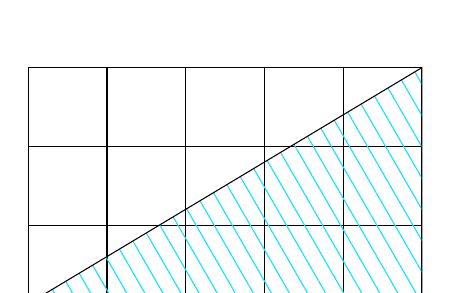
\begin{tikzpicture}
		\foreach \x in {1,2,3,4,5}
			\draw (\x,3)--(\x-1,3)--(\x-1,0)--(\x,0);
		\foreach \x in {1,2}
			\draw (0,\x)--(5,\x);
		\draw (5,3)--(5,0);
		\filldraw [pattern={Lines[angle=-60,distance={8pt/sqrt(2)}]},pattern color=Cerulean] (0,0)--(5,3)--(5,0)--cycle;
	\end{tikzpicture}
	\caption{A 3-by-5 rectangle sliced in half to create a triangle of half of the area.}
\end{figure}

\begin{figure}[htbp]
	\centering
	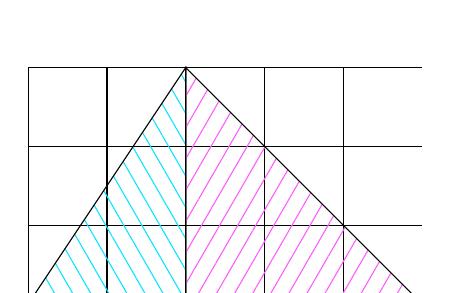
\begin{tikzpicture}
		\foreach \x in {1,2,3,4,5}
			\draw (\x,3)--(\x-1,3)--(\x-1,0)--(\x,0);
		\foreach \x in {1,2}
			\draw (0,\x)--(5,\x);
		\filldraw [pattern={Lines[angle=-60,distance={8pt/sqrt(2)}]},pattern color=Cerulean] (0,0)--(2,3)--(2,0)--cycle;
		\filldraw [pattern={Lines[angle=60,distance={8pt/sqrt(2)}]},pattern color=CarnationPink] (2,3)--(5,0)--(2,0)--cycle;
	\end{tikzpicture}
	\caption{A triangle different from that in Fig. 2 but still of the same base and height.}
\end{figure}

\begin{figure}[htbp]
	\centering
	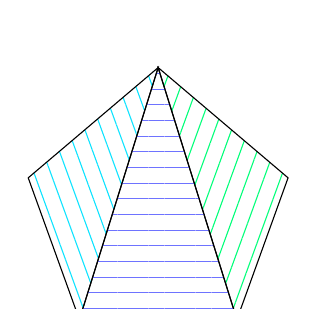
\begin{tikzpicture}
		\filldraw [pattern={Lines[angle=-70,distance={8pt/sqrt(2)}]},pattern color=Cerulean] (0,0)--(1,3.2)--(-0.65,1.8)--cycle;
		\filldraw [pattern={Lines[angle=70,distance={8pt/sqrt(2)}]},pattern color=JungleGreen] (2,0)--(2.65,1.8)--(1,3.2)--cycle;
		\filldraw [pattern={Lines[distance={8pt/sqrt(2)}]},pattern color=Periwinkle] (0,0)--(2,0)--(1,3.2)--cycle;
	\end{tikzpicture}
	\caption{A complex figure (a pentagon), subdivided into figures of known area.}
\end{figure}

\chapter{Further Operations}
\section{Exponents and Exponentiation}
\section{The Logarithm}
\section{Factorials}
\subsection{A Note on the Uncharted Path: Combinatorics}

\begin{advanced}
\chapter{Building Blocks of Higher-Level Mathematics: Set \mbox{Theory}}
\section{Sets and Useful Notation}
\section{How to Make Sets Marry: Union and Intersection}
\section{Mortal Enemies: Complements and Differences}
\section{A Justification for Proofs and Logic (Why You Should Care)}

\chapter{Functions}
\section{A Machine That Gives You Only One Result}
\section{Killing Everything As We Go: Surjective/Onto Functions}
\section{Loyalty: Injective/One-to-One Functions}
\section{A Backward Function...? Inverses and Pre-Images}

\chapter{The Flavour of Mathematical Analysis: Limits and the Infinitesimal}
\section{Are We There Yet? The Limit}
\section{Distances, Open Sets, and Numbers That Bind}
\section{How Far is Something? Metric Spaces}
\section{Closed Sets}
\section{Compact Sets}
\subsection{The Heine-Borel Theorem}
\section{A Long Chain: Sequences and Series}
\subsection{The Bolzano-Weierstrass Theorem}
\section{Useful Notation and Remarks on Their Intuition}
\section{Good Enough: Continuity and Continuous Functions}
\section{Real Numbers: Filling the Blanks}

\chapter{More on Geometry: Curves, Area, and Sums}

\chapter{Descending Down the Staircase: Derivation, the \mbox{Integral,} and the \mbox{Fundamental} Theorem of Calculus}
\section{Rates of Change}
\section{The Derivative}

\chapter{What Now?}
\section{Descriptions of Further Mathematics}
\subsection{Mathematical Analysis}
\subsection{Applied Mathematics}
\subsection{Algebra}
\subsection{Number Theory}
\subsection{Topology}
\subsection{Geometry}
\section{The Love of the Game}
\section{Competition Mathematics}
\section{A Final Remark}
\end{advanced}

\chapter{Solutions}
\section{Solutions to Chapter 1 Exercises}
\begin{enumerate}
	\item Any six counting numbers will do. An easy list is $\{1,2,3,4,5,6\}$.
	\item There is only one answer, and this is 0.
	\item Every single natural number is a whole number. Thus, there are infinite natural numbers that are whole numbers.
	\item See section 1.4.
	\item Every rational number can be written as a fraction, since a rational number is simply a fraction with integer entries for the numerator and denominator. However, not every fraction is a rational number; we simply need there to be a sufficiently `bad' numerator or denominator. In particular, we would like to put an irrational number for one of the two entries.
	\item Every rational number is able to be written as a decimal, since every rational number is a fraction and every fraction can be written as a decimal. However, not every decimal can be written as a rational number, since some decimals cannot be written as a fraction composed of integers, and that means that they cannot be rational numbers, by definition.
\end{enumerate}
\end{document}